\chapter{Ergebnisse}   \label{ch_4}
Im folgenden Kapitel werden die durchgeführten statistischen Berechnungen dargestellt. Zu Beginn werden die deskriptiven Ergebnisse beschrieben und mit den Normwerten verglichen, woraufhin die statistische Überprüfung der Manipulation folgt. Im inferenzstatistischen Unterkapitel wird mit der Prüfung der Vorraussetzung der einzelnen Test mathematisch dargestellt und abschließend werden die Ergebnisse der drei Hypothesen präsentiert. Die ausführliche Interpretation der Ergebnisse geschieht im nachkommenden Kapitel ~\ref{ch_5}.

\section{Deskriptive Ergebnisse}    \label{sec_4.1}
Die Fallvignetten wießen, bei einem $Min$~=~1 und einem $Max$~=~101, einen Mittelwert von $M$~=~26.46 ($SD$~=~27.98) auf. Der Median lag bei $Mdn$~=~19. Bei einer Schiefe von 1.17 und Kurtosis von 0.53, liegt eine rechstschiefe bzw. linkssteile und steilgipflige Verteilung vor. Abbildung~\ref{Histogramm VicBlame} stellt die multimodale Verteilung der Verantwortungszuschreibung bildlich da. %Aus dem Boxplot sind zudem ein paar milde Ausreißerwerte zu entnehmen.
% Modus
\begin{figure}[htb]
    \centering
        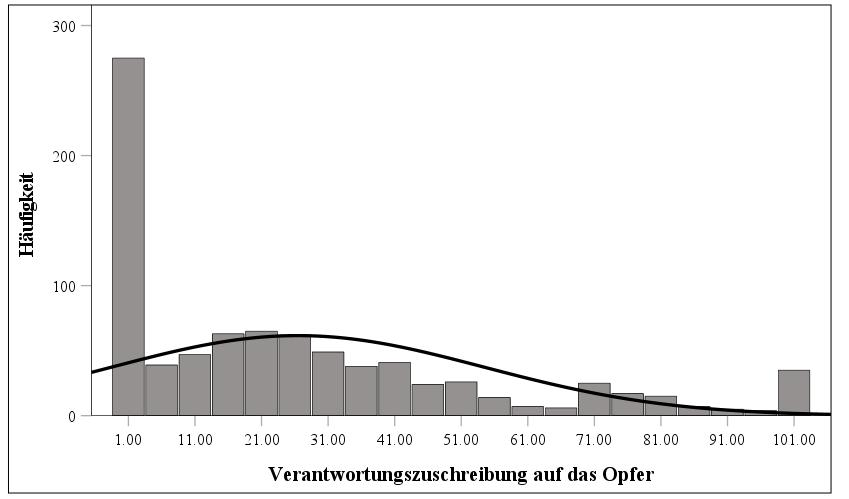
\includegraphics[width=0.8\linewidth]{Histogramm VicBlame.jpg}
        \caption[Histogramm Verantwortungszuschreibung]{Verteilung der Verantwortungszuschreibung.}
        \label{Histogramm VicBlame}
\end{figure}



Der DVMAS zeigte einen Mittelwert von $M$~=~2.60 ($SD$~=~0.80) und einen Median von $Mdn$~=~2.5. Der geringste Wert war dabei $Min$~=~1 und der höchsete $Max$~=~5.56. Eine Schiefe von 0.60 bildet eine leicht rechstschiefe Verteilung. Die Kurtosis von 0.09 bildet eine leicht steilere Verteilung, als die Normalverteilung. Beide Werte weichen demzufolge leicht von einer Normalverteilung ab. Die Abbildung~\ref{Histogramm DVMAS} bildet die beschriebenen Werte bildlich ab. %Aus dem Boxplot sind zudem ein paar milde Ausreißerwerte zu entnehmen.
% Normwerte
% Modus
\begin{figure}[htb]
    \centering
        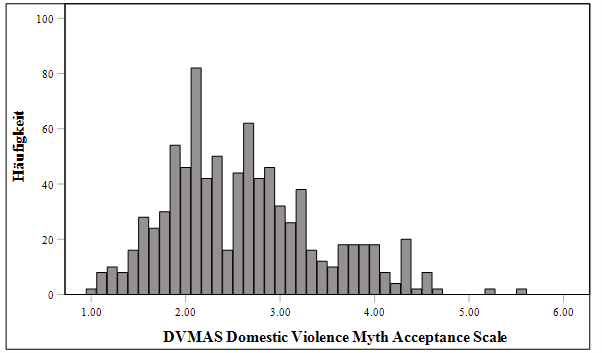
\includegraphics[width=0.8\linewidth]{Histogramm - DVMAS.png}
        \caption[Histogramm Altersverteilung]{Verteilung der Akzeptanz von Gewaltmythen.}
        \label{Histogramm DVMAS}
\end{figure}



Beim Deutschen Aggressionsfragebogen wurde ein Mittelwert von $M$~=~1.88 ($SD$~=~0.43) und ein Median von $Mdn$~=~1.79 berechnet. Der geringste angegebene Wert betrug $Min$~=~1.10 und der höchste $Max$~=~3.52. Die Verteilung wies einen Schiefe von 0.94 und eine Kurtosis von 0.88 auf. Demzufolge ist die Verteilung rechstschiefe und hat eine breitgipflige Form, sowie eine Multimodalität. In Abbildung~\ref{Histogramm AggroFB} ist eine bildliche Darstellung der Verteilung zu sehen.
\begin{figure}[htb!]
    \centering
        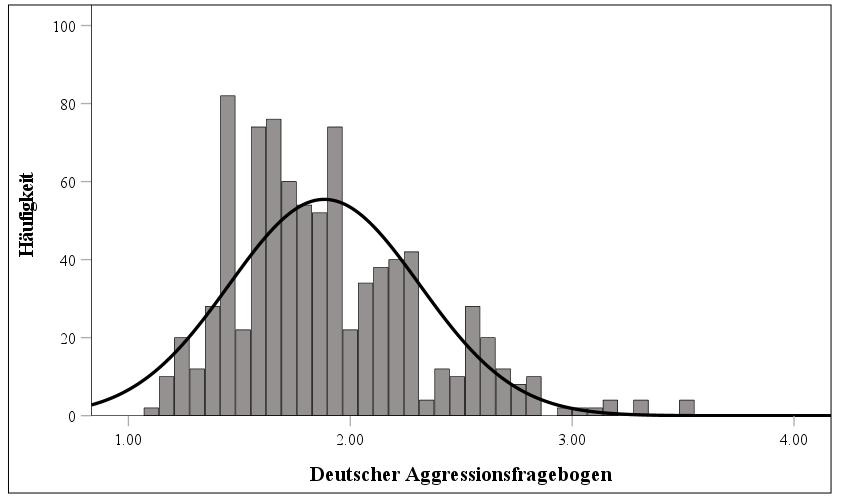
\includegraphics[width=0.8\linewidth]{Histogramm AggroFB.jpg}
        \caption[Histogramm Aggressionsfragebogen]{Verteilung der Angaben des Aggressionsfragebogens.}
        \label{Histogramm AggroFB}
\end{figure}


% Ausreißer
% Normwerte
% Modus


\section{Manipulationscheck}    \label{sec_4.2}
dd


\section{Inferenzstatistische Ergebnisse}    \label{sec_4.3}
Ergebnisse der Hypothesentests


\subsection{Hypothese 1}    \label{subsec_4.3.1}
hier Vorraussetzungsergebnisse statistisch darlegen
% https://www.youtube.com/watch?v=ZPoYMfx0aIY (Vorraussetzung für Pearson)


\subsection{Hypothese 2}    \label{subsec_4.3.2}
hier Vorraussetzungsergebnisse statistisch darlegen
% https://www.youtube.com/watch?v=ZPoYMfx0aIY (Vorraussetzung für Pearson)


\subsection{Hypothese 3}    \label{subsec_4.3.3}
hier Vorraussetzungsergebnisse statistisch darlegen

Moderation: 14.31\% der Varianz des DVMAS werden durch das Modell erklärt.
Modell erklärt tatsächlich etwas, weil p kleiner .01 ist.
Grüne Linie: Geschlecht sorgt für höheren DVMAS-Wert bei gleichbleibender Aggression. Bei gleichbleibendem Aggressions-Score sorgt das Geschlecht für einen höheren DVMAS-Wert.

einen haupteffekt der signifikant ist der andere nicht, so wie die interaktion. Regressionsmodell mit 3 Prediktoren. eins hat n sig. Gewicht, der andere nicht.

Da die obere Grenze einen größeren Wert als 0 aufweist, ist die Interaktion nicht signifikant.

Eine Moderationsanalyse wurde durchgeführt, um zu bestimmen, ob die Interaktion zwischen Alter und Freizeit die Nutzung von sozialen Medien signifikant vorhersagt. Die Ergebnisse konnten keinen Moderationseffekt von Alter auf die Beziehung zwischen Freizeit auf Social Media-Nutzung finden, $\Delta R^{2}$ = 16.47\%, F(1, 96) = 18.93, p = .241, 95\% CI[-0.047, -0.015].


\section{Explorative Ergebnisse}    \label{sec_4.4}

